\section{实验总结}
\subsection{FPGA 资源利用情况}

本项目共占用 FPGA 逻辑资源 21\%,内存资源 48\%,均在合理范围内。

\begin{figure}[H]
    \centering
    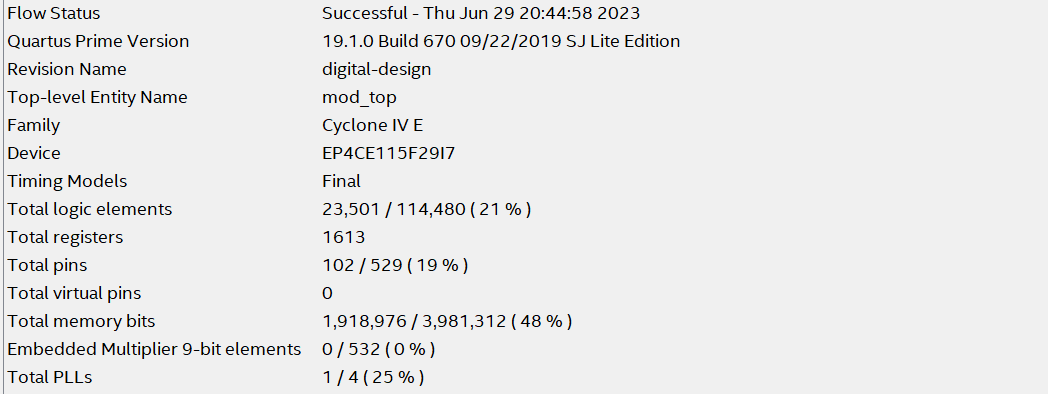
\includegraphics[scale=0.82]{images/compile_result.png}
    \caption{FPGA 资源利用情况}
    \label{fig:compile_result}
\end{figure}


% \subsection{未来工作}
% 这部分保留还是去掉?

\subsection{总结与心得}
本次项目中,我们预先设计了较为完整的文件框架,将项目各功能分开封装处理,提前写好模块接口,同时维护了比较细节的 README 文件,这帮助我们在开发时保持有序,大大提高了开发效率。

实际开发时,由于本学期课业紧张,我们并没有太多富余的时间,这使得我们工期一度吃紧。这值得我们在时间分配问题上作出反思,日后做到合理地配置,而非逐个赶工。不过受益于良好的项目框架管理,且我们及时调整了项目计划目标,砍掉了一些过于复杂的初期设想,最后还是很好地完成了预期的游戏功能。

开发过程中,我们保障了比较充足的实验室测试时间,尤其是输出部分,做到随写、随测、随修(debug),同时及时获取进度快的同学与助教老师的帮助,这些都帮助了我们快速、可靠地完成项目。

此外,这次开发使我们亲身体会了硬件语言的特殊性,如时序分析、时序逻辑特殊语法、组合逻辑必须覆盖所有情况等要求,这帮助我们拓宽了对编程语言的认识,同时深化了对课上所学数字逻辑的理解。

最后,感谢不辞辛劳的老师和助教的鼓励与帮助。